%%%%%%%%%%%%%%%%%%%%%%%%%%%%%%%%%%%%%%%%%%%%%%%%%%%%%%%%%%%%%%%%%%%%%%%
% Based on IEEE the conference template available                     %
% at https://www.ieee.org/conferences/publishing/templates.html       %
% Adapted for the Data Science Lab course at Politecnico di Torino    %
% by Giuseppe Attanasio, Flavio Giobergia                             %
% 2020, DataBase and Data Mining Group                                %
%%%%%%%%%%%%%%%%%%%%%%%%%%%%%%%%%%%%%%%%%%%%%%%%%%%%%%%%%%%%%%%%%%%%%%%

\documentclass[conference]{IEEEtran}
\usepackage{cite}
\usepackage{amsmath,amssymb,amsfonts}
\usepackage{algorithm}
\usepackage{algorithmic}
\usepackage{graphicx}
\usepackage{textcomp}
\usepackage{xcolor}
\usepackage{subfigure}

\begin{document}

\title{
Lab L7: Epidemic processes
}

\author{
    \IEEEauthorblockN{Emanuele Pietropaolo}
    \IEEEauthorblockA{
        \textit{Politecnico di Torino} \\
        Student id: s319501 \\
        emanuele.pietropaolo@studenti.polito.it
        }
}

\maketitle
\begin{abstract}
    
\end{abstract}

\section{Problem overview}

\section{Proposed approach}

    \subsection{The unfolding of events}

    \subsection{Simulation parameters}
   
\section{Results}

    % \begin{table}[!ht]
    %     \centering
    %     \caption{Average time to reach consensus with $n = 1000$ and $p_1=0.51$}
    %     \label{tab:all_graphs}
    %     \begin{tabular}{|c|c|c|c|}
    %     \hline
    %             & ER       & Z2        & Z3       \\ \hline
    %     Time & 589,1798 & 2054,6865 & 856,7241 \\ \hline
    %     \end{tabular}
    % \end{table}
    

    \subsection{Erdős Rényi graphs} 

        % \begin{figure}[!ht]
        %     \centering
        %     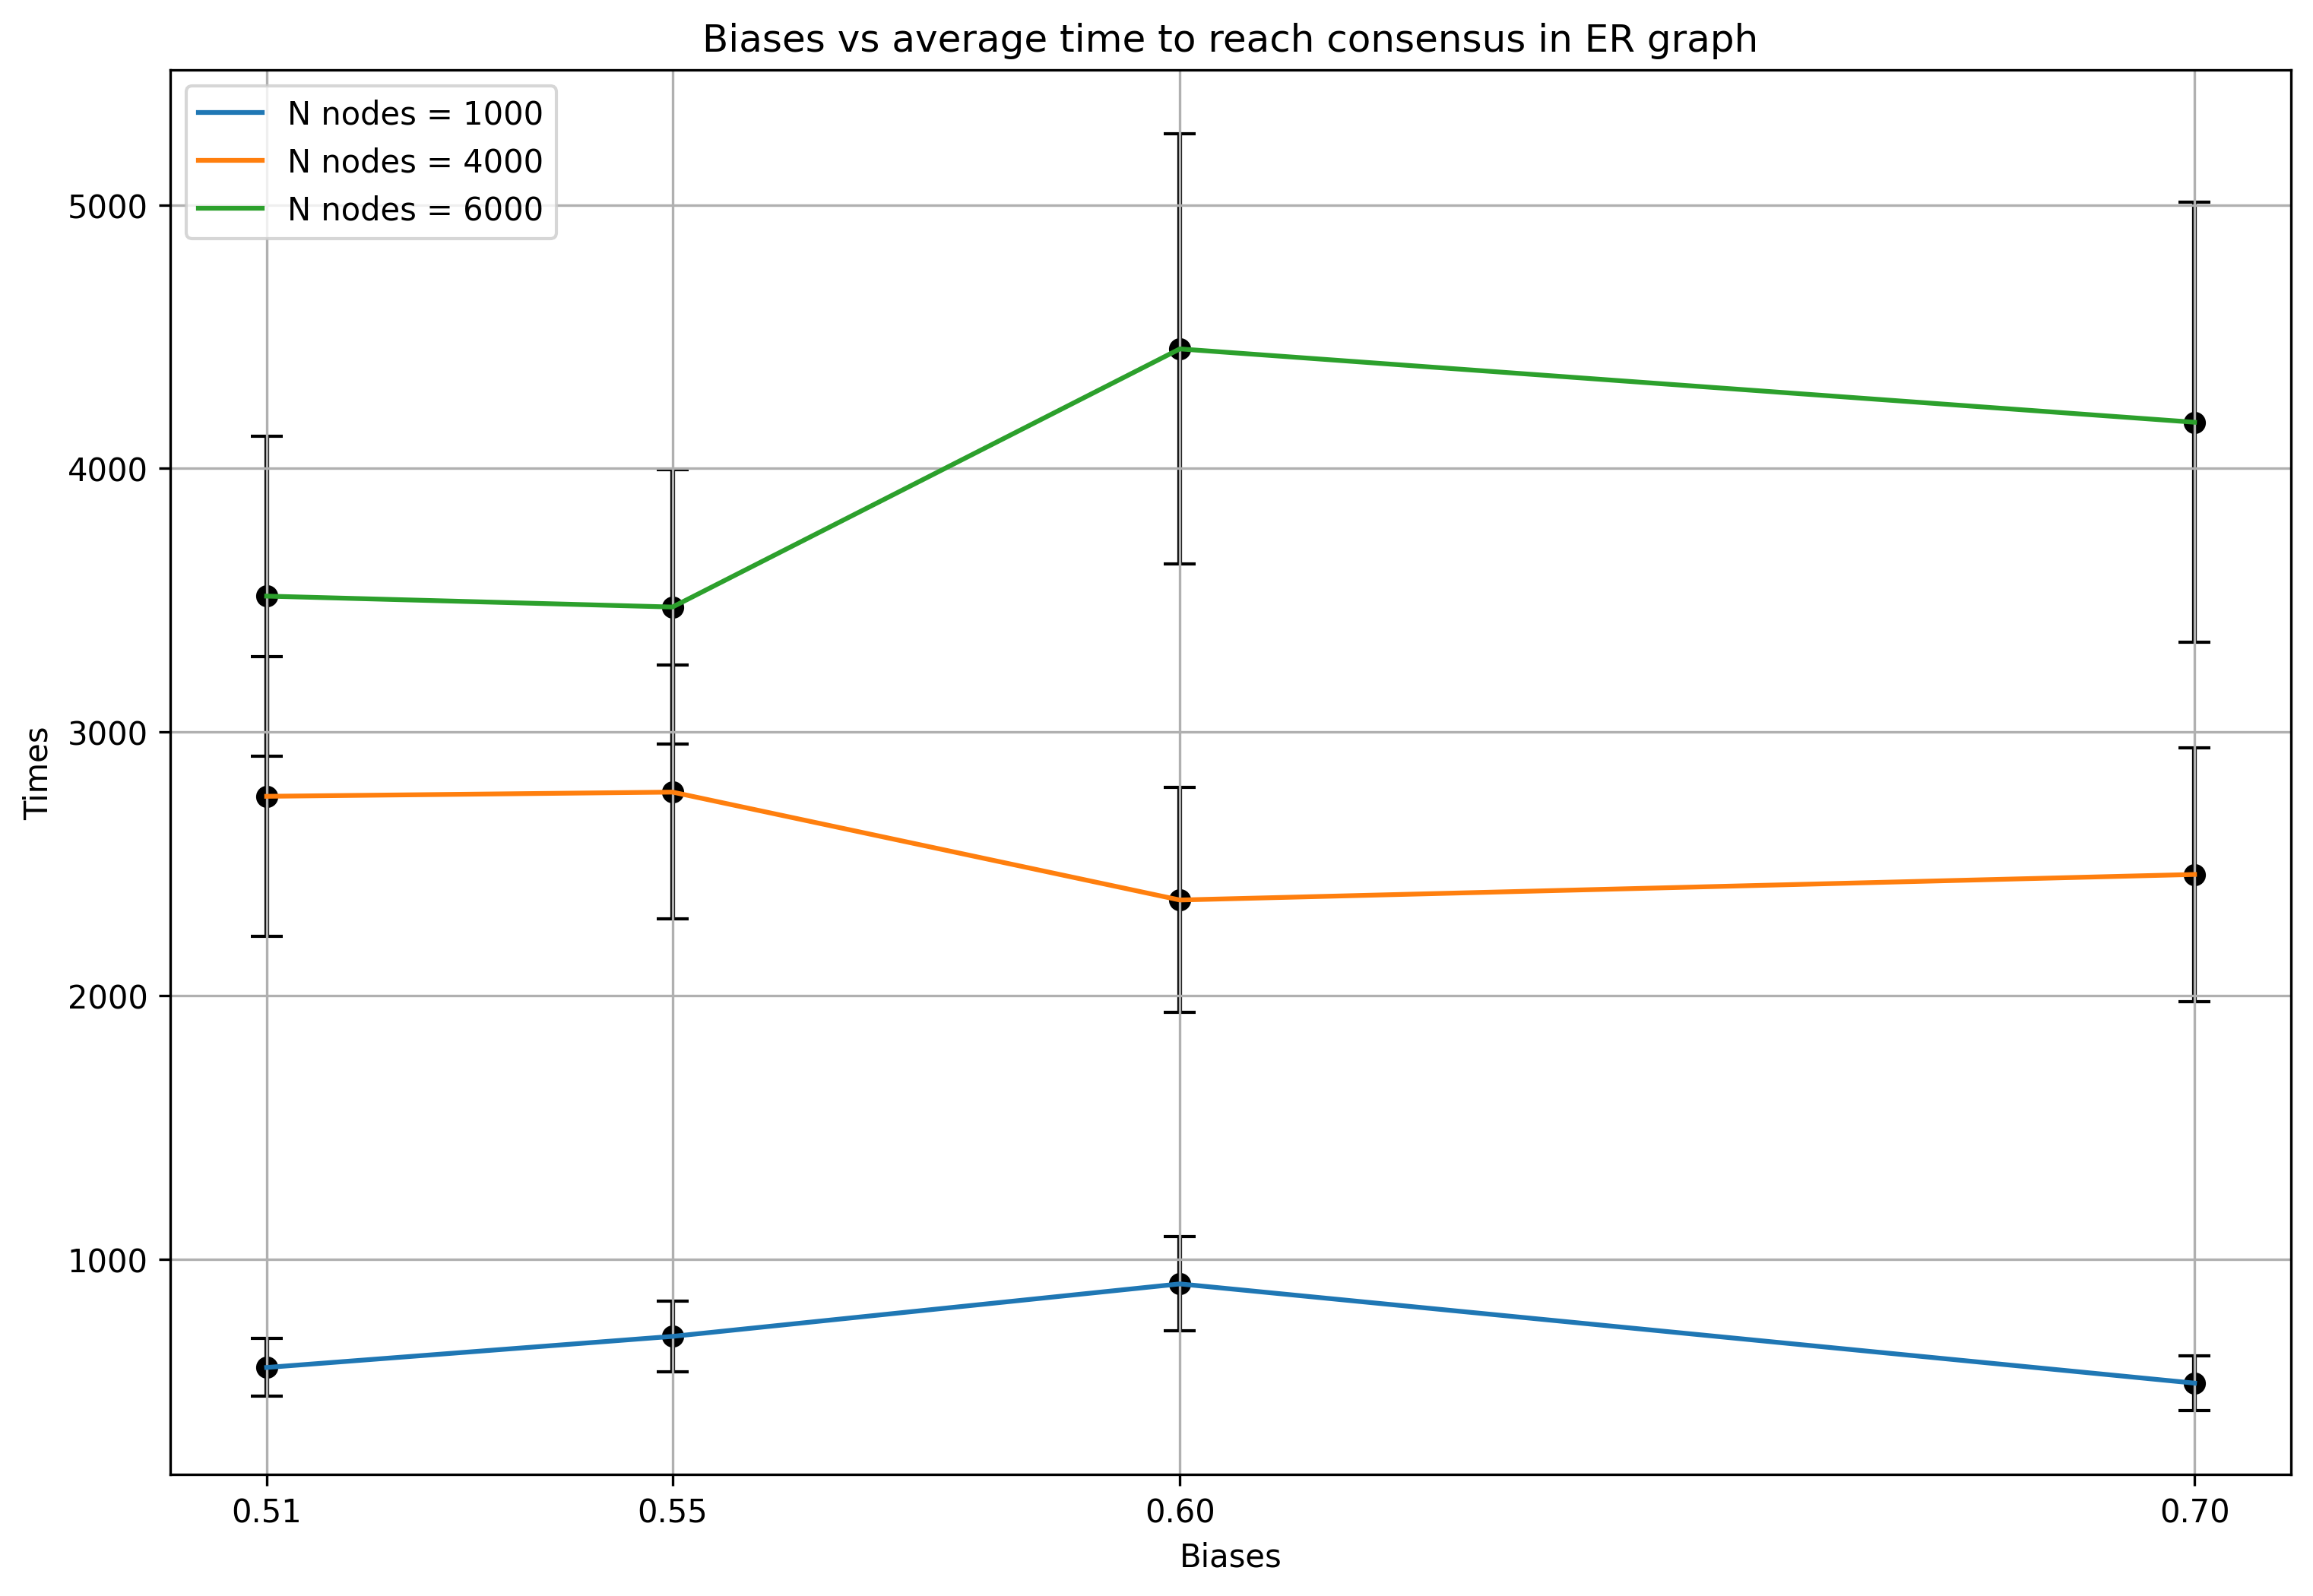
\includegraphics[width=\columnwidth]{media/er_times.png}
        %     \caption[short]{Average time to reach consensus based on different bias probability}
        %     \label{fig:er_times}
        % \end{figure}

        %Looking at this graph, it can be observed that the differences between the various groups (N nodes = 1000, N nodes = 4000, N nodes = 6000) are not distinct enough to be attributed to reasons other than normal random variation. The lines representing each group intersect and overlap at several points on the graph, indicating that there is no clear separation or significant difference in their +1 probability as bias probability changes. This suggests that the variations observed in the +1 probability across different bias probabilities for each group could be due to inherent randomness in the system rather than any systematic differences between the groups. In other words, the graph does not provide strong evidence to suggest that the number of nodes in the graph has a significant impact on the +1 probability at different bias probabilities. It’s important to note, however, that this interpretation is based on the visual inspection of the graph and a more rigorous statistical analysis may be required to confirm these observations

\section{Conclusion}

%\bibliography{bibliography}
%\bibliographystyle{ieeetr}

\end{document}
